\chapter{Modeling and model evaluation}
\label{sec:data_preparation}

\section{Preliminary operations}
First steps in this part of the modeling was to split our dataset in a train set, used to train every model, and a test set, to compute the evaluation metrics of them.\\
Then, to avoid bias due to the unbalanced target classes, we did an oversampling over the sets using the SMOTE technique.
Finally, we have built many models, with an iterative approach over each one to find a proper parameters setting that could achieve good results.
\subsection{Decision Tree Classifier}
A Decision Tree is a supervised learning model that employs a hierarchical structure of nodes to make decisions based on input features. Each internal node represents a feature, and the branches represent possible outcomes based on the feature's value. Decision Trees excel in capturing complex relationships and are easy to interpret. However, they are prone to overfitting and can struggle with handling continuous data or outliers.\subsection{Random Forest}
The Random Forest algorithm is an ensemble learning method that combines multiple decision trees to make predictions. It generates a multitude of decision trees and aggregates their outputs to produce a final prediction. Random Forests are known for their robustness, versatility, and resistance to overfitting. They are particularly effective for handling high-dimensional data and are widely used for classification and regression tasks
\subsection{Gradient Boosting Classifier}
Gradient Boosting is an ensemble learning technique that combines multiple weak learners, typically decision trees, to create a strong predictive model. It works by iteratively training new models that focus on the errors made by the previous models, gradually reducing the overall error. Gradient Boosting is highly effective in handling tabular data and has achieved remarkable success in various machine learning competitions.

\subsection{AdaBoost Classifier}
Adaboost, short for Adaptive Boosting, is another ensemble learning method that sequentially combines weak learners to create a strong predictive model. It assigns higher weights to misclassified instances in each iteration, enabling subsequent models to focus on those instances. Adaboost is versatile, relatively easy to implement, and can be used for both classification and regression tasks. However, it is sensitive to noisy data and outliers.
\subsection{Gaussian Naive Bayes Classifier}
Gaussian Naive Bayes is a probabilistic classifier that applies Bayes' theorem with the assumption of independence between features. It assumes that the features follow a Gaussian distribution and calculates the probability of each class given the observed feature values. Despite its simplicity, Gaussian Naive Bayes can perform well in many real-world applications, especially when the independence assumption holds.
\subsection{K-Neighborhood classifier}
K-Nearest Neighbors is a non-parametric algorithm used for both classification and regression tasks. It classifies new instances by finding the closest labeled instances in the feature space and assigning the majority class or predicting the average value of their targets. KNN is easy to understand and implement, but it can be computationally expensive, especially with large datasets. It is also sensitive to the choice of the number of neighbors (K) and the distance metric.
\subsection{Support Vector Classifier}
Support Vector Machine is a powerful supervised learning algorithm that separates data points into different classes by constructing hyperplanes in a high-dimensional feature space. It aims to find an optimal hyperplane that maximizes the margin between classes while minimizing classification errors. SVMs can handle both linear and non-linear data through the use of kernel functions. They are effective in high-dimensional spaces and have good generalization capabilities. However, they can be sensitive to the choice of hyperparameters and require careful preprocessing of data.

\section{Train and test splits and oversampling}
The dataset used in this project was divided into a 70\% training set and a 30\% testing set. This split ensured that a substantial portion of the data was dedicated to training the machine learning models, while also providing an independent subset for evaluating their performance.

Furthermore, it was observed that the dataset exhibited class imbalance, where the minority class had significantly fewer instances compared to the majority class, \textbf{HIGH} class have very few instances compared to \textbf{LOW and MEDIUM}. To address this issue and ensure fair representation of all classes during model training, oversampling techniques were applied.

Specifically, oversampling was performed for the minority class using the BorderlineSMOTE method.
\subsection{BorderlineSMOTE}
BorderlineSMOTE generates synthetic samples for the minority class, effectively increasing its representation in the dataset. By incorporating these synthetic samples, the training data became more balanced, allowing the models to learn from both the majority and minority classes more effectively.

By splitting the data into training and testing sets and applying oversampling techniques, we aimed to improve the robustness and performance of the machine learning models, particularly in handling class imbalance challenges. The resulting datasets were then used to train and evaluate the models, providing a comprehensive assessment of their effectiveness in addressing the problem at hand.
\section{Parameter tuning}
We wanted to see how different machine learning models perform without changing their default settings. We thought about tweaking the parameters to potentially improve the models, but we hit a roadblock. The problem was that our resources, like computing power and time, weren't enough to handle the long runtimes that come with parameter tuning.

Even though we couldn't fine-tune the models as much as we wanted, we still went ahead and evaluated them using their default configurations.

In our quest for finding the optimal configuration for the Random Forest model, we enlisted the help of sklearn's random search cross-validation (CV) technique. This approach allowed us to explore different combinations of parameters in a randomized manner, hoping to strike gold with a winning combination.

However, despite our efforts, the results didn't quite meet our expectations. The random search CV didn't yield a significant number of promising outcomes that would greatly enhance the model's performance on our specific dataset.

\section{Model Evaluation}
\begin{figure}[h!]
    \centering
    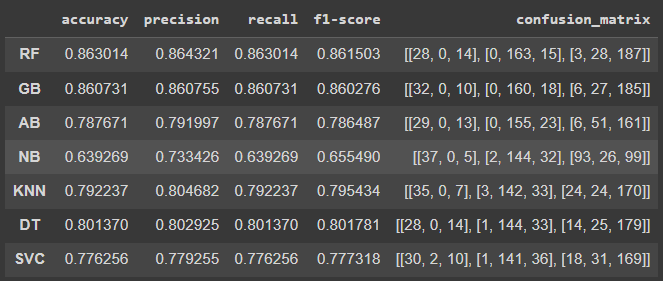
\includegraphics[width=0.8\textwidth]{imgs/initial_results.png}
    \caption{Models initial results}
    \label{fig:results}
\end{figure}
The Random Forest and Gradient Boosting models showed similar and consistent results across accuracy, precision, recall, and F1-score. These models demonstrated balanced and robust performance with relatively few misclassifications, as evident from the confusion matrices.

On the other hand, the Adaboost model had slightly lower values for accuracy, precision, recall, and F1-score compared to the Random Forest and Gradient Boosting models. It faced challenges in correctly classifying instances, particularly in the minority class.

The Gaussian Naive Bayes model achieved the lowest accuracy among all models, indicating a lower overall correctness in its predictions. Although it had relatively high precision for positive instances, it struggled with recall, resulting in a higher number of false negatives. The confusion matrix revealed significant misclassifications, particularly in the minority class.

The K-nearest Neighbors and Decision Tree models exhibited similar performance with reasonably good accuracy, precision, recall, and F1-score. The confusion matrices indicated some misclassifications across the classes, but overall, these models performed adequately.

In contrast, the Support Vector Classifier model had lower accuracy compared to most other models. The precision, recall, and F1-score aligned with the accuracy, suggesting a moderate performance. The confusion matrix highlighted misclassifications, especially with false positives in the majority class.

\begin{figure}[h!]
    \centering
    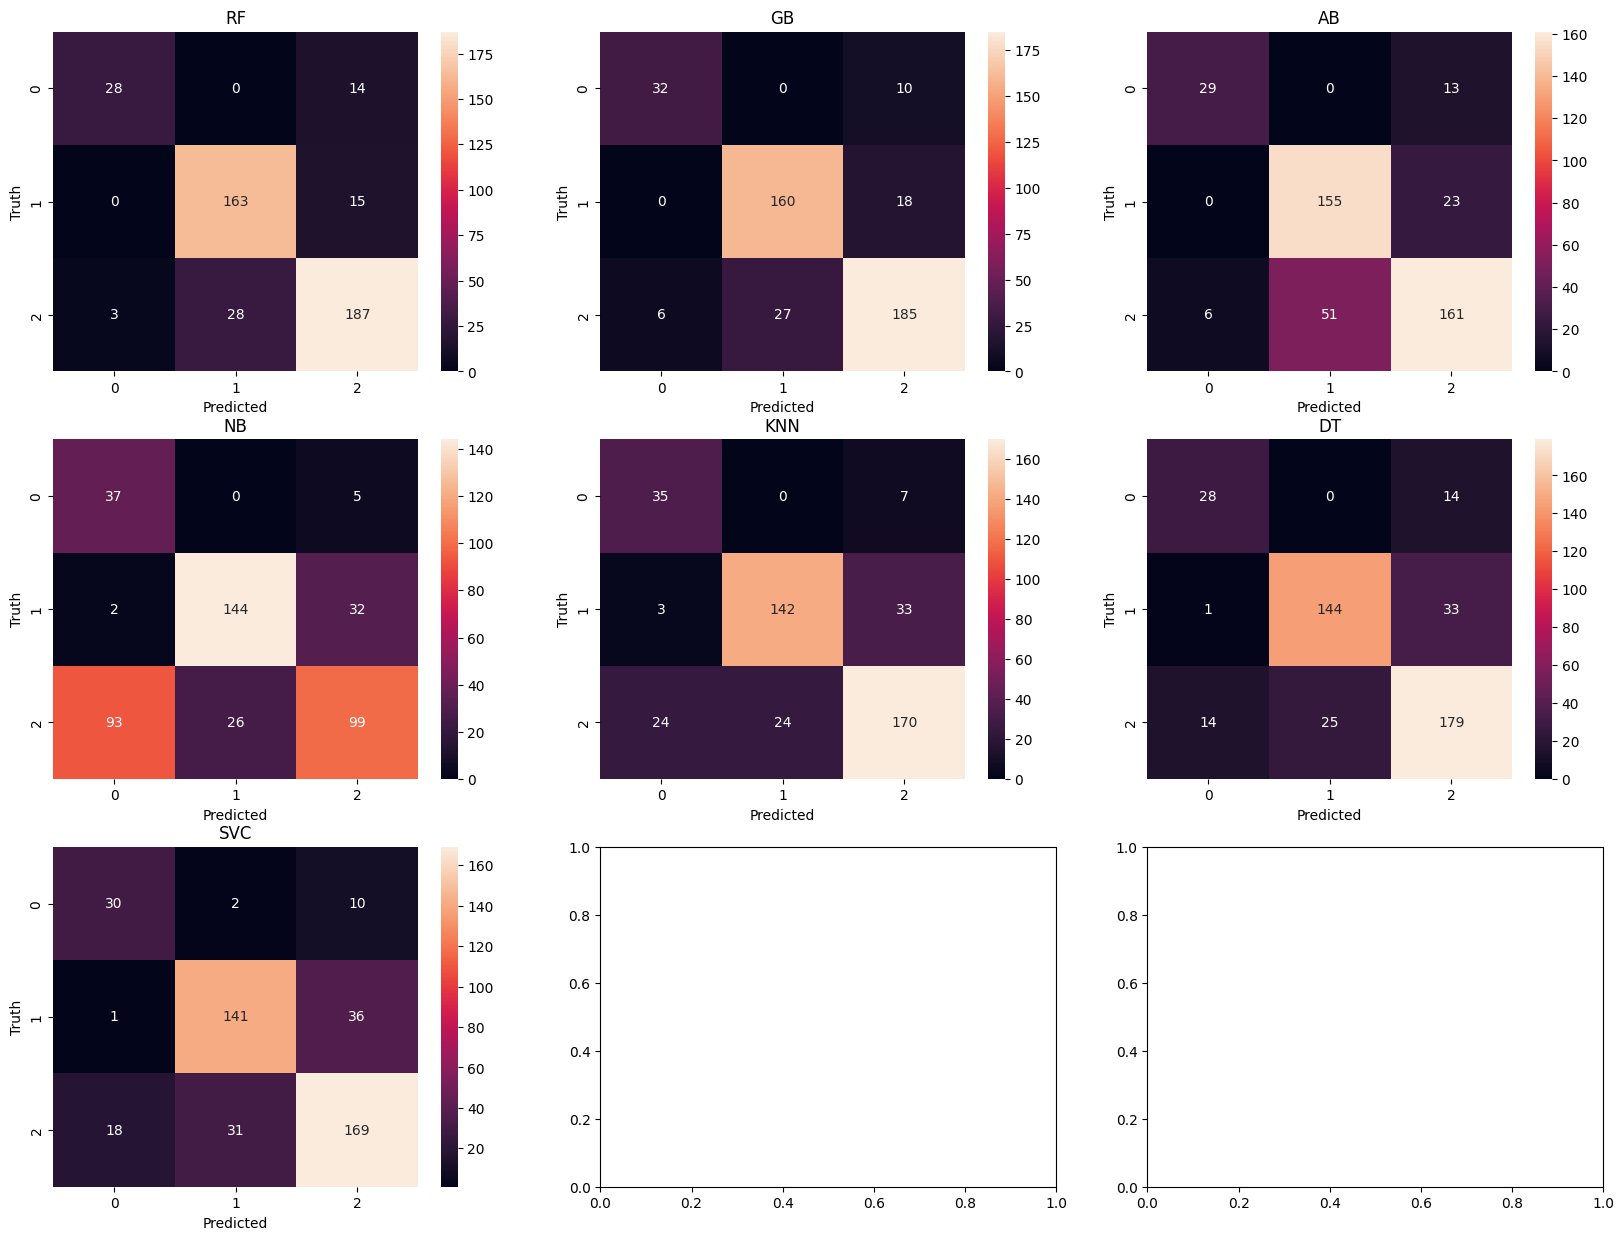
\includegraphics[width=0.8\textwidth]{imgs/confusion matrix.png}
    \caption{Confusion Matrix}
    \label{fig:ConfusionMatrix}
\end{figure}

\subsection{K-fold cross-validation}
KFold is a technique used in machine learning for cross-validation. It involves splitting the dataset into k equal-sized folds or subsets. The model is then trained and evaluated k times, each time using a different fold as the validation set and the remaining folds as the training set. This ensures that each data point is used for both training and validation, providing a more reliable estimation of the model's performance.

cross\_val\_score is a function provided by the scikit-learn library that automates the process of performing KFold cross-validation and computing evaluation metrics. It simplifies the process by allowing you to specify the number of folds (k) and the evaluation metric of interest, such as accuracy or mean squared error. The function takes care of splitting the data, training the model, and evaluating its performance on each fold. It returns an array of scores, representing the performance metric for each fold.

In our project, we utilized KFold cross-validation along with cross\_val\_score to assess the performance of our machine learning models. By employing this technique, we were able to obtain a more robust evaluation of the models, taking into account variations in performance across different subsets of the data. This helped us gain a better understanding of how well our models generalize to unseen data and allowed us to make more informed decisions about their effectiveness.

\begin{figure}[h!]
    \centering
    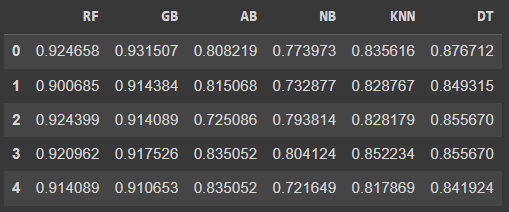
\includegraphics[width=0.8\textwidth]{imgs/kfold_1.png}
    \caption{K-fold cross-validation}
    \label{fig:K-fold cross-validation}
\end{figure}

\begin{figure}[h!]
    \centering
    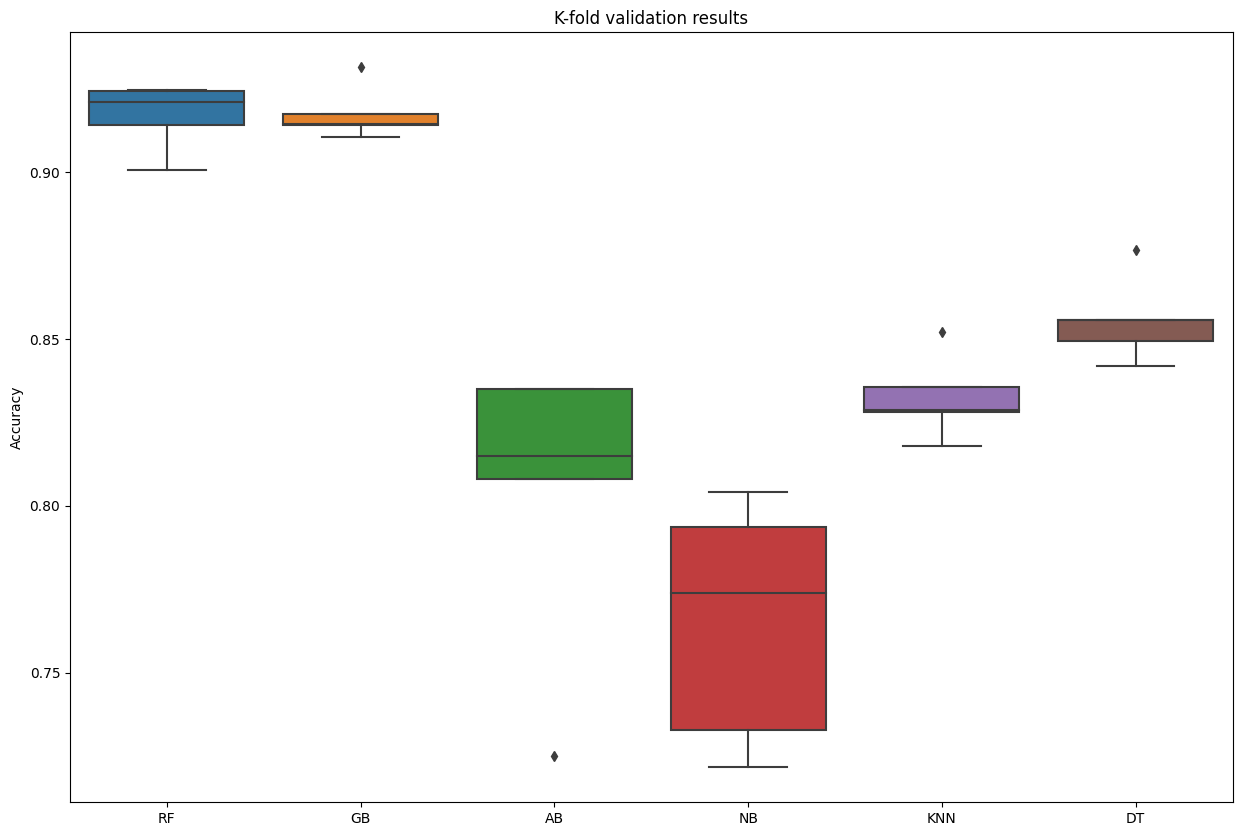
\includegraphics[width=0.8\textwidth]{imgs/kfold_box.png}
    \caption{K-fold box plot}
    \label{fig:K-fold box}
\end{figure}

Analyzing the scores, we can observe the following:
\begin{itemize}
    \item  Random Forest (RF) and Gradient Boosting (GB) consistently achieved high scores across all folds, indicating strong performance and good generalization ability. These models consistently outperformed the other models in terms of accuracy.
    \item Adaboost (AB) had relatively lower scores compared to RF and GB, but it still displayed decent performance across most folds. It showed some variability in performance, with scores ranging from moderate to good.
    \item Gaussian Naive Bayes (NB) had mixed performance, with scores varying across folds. It achieved relatively lower scores compared to RF, GB, and AB, indicating that it struggled to capture the complexities of the dataset.
    \item K-nearest Neighbors (KNN),Decision Tree (DT) and Support Vector Classifier (SVC) models had scores that varied across folds but generally performed at a moderate level. They were outperformed by RF, GB and SVC but showed comparable performance to AB and NB.
\end{itemize}

We can see that Random Forest and Gradient Boosting have the most consistent performance across all folds, with scores ranging from good to excellent. They also achieved the highest accuracy among all models, indicating that they were able to correctly classify the majority of instances in the dataset. These models demonstrated strong generalization ability, suggesting that they would perform well on unseen data.

\section{Feature Selection | SelectKBest}
SelectKBest is a feature selection algorithm that selects the best features from a dataset based on univariate statistical tests. It can be used for classification or regression problems. The algorithm works by scoring each feature based on a statistical test, such as the chi-squared. It then selects the top k features with the highest scores.

We tried to prune the model selecting the best features, but we didn't get any significant results. The model performed better with all the features we selected in the first place.

\textit{We left the code in the notebook for reference.}

\section{ROC Curve}
The ROC curve is like a graph that shows how well a machine learning system can tell things apart. It plots the true positive rate (how well it detects the right things) against the false positive rate (how often it makes mistakes) as we change the threshold for making decisions. The curve shows how the sensitivity (ability to detect) changes as the fall-out (making mistakes) varies.

Basically, if we know the probabilities of detecting something and making a mistake, we can create the ROC curve by looking at the cumulative probabilities. We plot the detection probability on the y-axis and the false-alarm probability on the x-axis.
It helps us see how well a classifier can distinguish between positive and negative cases. We can look at the shape of the curve and the area under it to evaluate the performance. A larger area under the curve means a better classifier that can tell things apart more accurately.
So it is a handy way to measure how well a classifier can do its job. It lets us compare different models and see how good they are at separating the good from the bad.

\begin{center}

    \begin{figure}[h!]
        \centering
        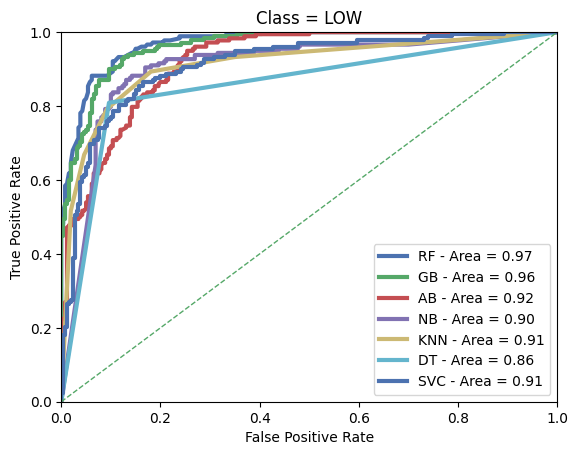
\includegraphics[width=0.8\textwidth]{imgs/roc low.png}
        \caption{ROC Curve - LOW}
        \label{fig:ROC LOW}
    \end{figure}
    \begin{figure}[h!]
        \centering
        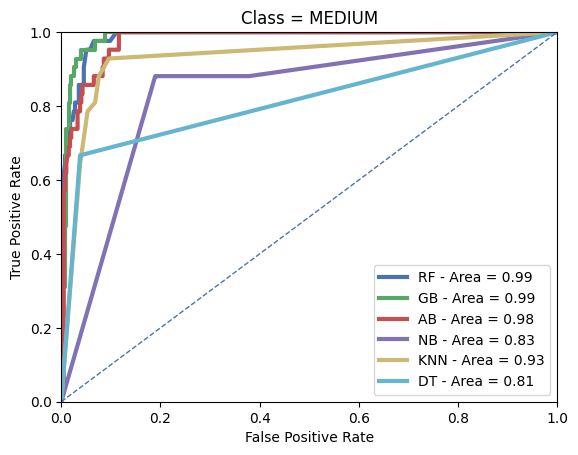
\includegraphics[width=0.8\textwidth]{imgs/roc medium.png}
        \caption{ROC Curve - Medium}
        \label{fig:ROC ALL}
    \end{figure}
    \begin{figure}[h!]
        \centering
        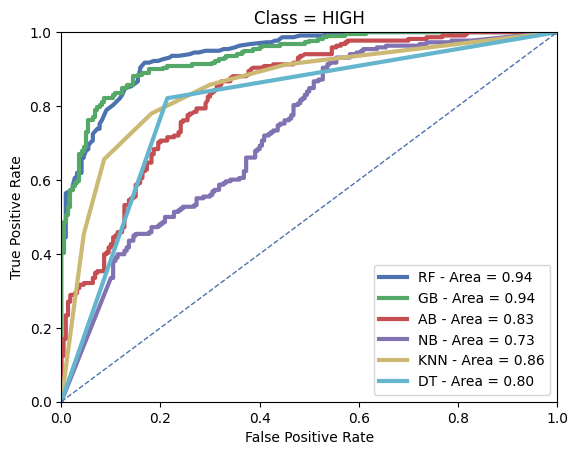
\includegraphics[width=0.8\textwidth]{imgs/roc high.png}
        \caption{ROC Curve - HIGH}
        \label{fig:ROC HIGH}
    \end{figure}
\end{center}
\clearpage

\subsection{Performance}
In the \textbf{medium category}, the Random Forest (RF), Gradient Boosting (GB) and AdaBoost (AB) models exhibit excellent performance with AUC scores of 0.99, 0.99 and 0.98, respectively. These models demonstrate strong discrimination between classes, making them reliable choices for accurate classification tasks.

In the low category, the Gradient Boosting (GB) and Random Forest (RF) models stand out with a promising AUC score of 0.97 and 0.96 each. These are suitable option for classification tasks where accuracy is crucial.

In the high category, both the Random Forest (RF) and Gradient Boosting (GB) models shine with AUC scores of 0.94. These models demonstrate robust predictive capabilities and strong discrimination between classes. Additionally, the AdaBoost (AB) model performs reasonably well with an AUC score of 0.83.

The Gaussian Naive Bayes (NB) model achieves relatively lower AUC scores across all categories, suggesting limitations in accurately distinguishing between classes. However, it still demonstrates moderate performance, especially in the medium and low categories.

Sp, in the end, the Random Forest (RF) and Gradient Boosting (GB) models consistently showcase top-tier performance across different performance categories, making them the best models among those evaluated.

\section{Considerations on Neural Networks}
Although they are not the main focus of the project, we have made some test using neural networks. However, results were not great and we preferred to put more effort on other models, leaving them out of our work.
We tried to tune the parameters of the network with some techniques, but we just achieved long training times and low results.
Due to that, we also preferred not to put the code into the final version of the project to avoid slow-downs on time consuming operations during the notebook execution derived from those tests.
\section{Final considerations}
Our overall goals of models with pretty good metrics have been achieved with many different models. Furthermore, we had the chance to practice data and machine learning techniques and discover a lot of new technologies that are surely going to be useful in our future. We also had the chance to work with a real dataset and understand how to deal with it, from the data cleaning to the final model evaluation.